\clearpage
\section{Temporal Alternating Direction Method of Multipliers (tADMM)}

\subsection{LinDistFlow MPOPF with tADMM}

\subsubsection{Problem Overview}

The Temporal ADMM (tADMM) algorithm decomposes the multi-period optimal power flow problem for distribution networks into $T$ subproblems, each corresponding to one time period. This formulation uses the linearized DistFlow model to capture network physics including voltage drops and reactive power flows.

\subsubsection{Variable Color Coding}
\begin{itemize}
    \item $B_j^{t_0}[t]$: Local SOC variables for battery $j$ in subproblem $t_0$, evaluated at time $t$
    \item $\hat{B}_j[t]$: Global consensus SOC for battery $j$ at time $t$
    \item $u_j^{t_0}[t]$: Local scaled dual variables for battery $j$ in subproblem $t_0$, for time $t$
\end{itemize}

\subsubsection{Sets and Indices}
\begin{itemize}
    \item $\mathcal{N}$: Set of all nodes (buses)
    \item $\mathcal{L}$: Set of all branches (lines)
    \item $\mathcal{L}_1$: Set of branches connected to substation (node 1)
    \item $\mathcal{B}$: Set of nodes with batteries
    \item $\mathcal{D}$: Set of nodes with PV (DER)
    \item $\mathcal{T} = \{1, 2, \ldots, T\}$: Set of time periods
    \item $t_0 \in \mathcal{T}$: Index for a specific time period in tADMM decomposition
    \item $j \in \mathcal{N}$: Node index
    \item $(i,j) \in \mathcal{L}$: Branch from node $i$ to node $j$
\end{itemize}

\subsubsection{tADMM Algorithm Structure}

The algorithm alternates between three update steps:

\paragraph{Step 1: Subproblem Update}
For each subproblem $t_0 \in \{1, 2, \ldots, T\}$:

\begin{align}
\min_{\substack{P_{\text{Subs}}^{t_0}, Q_{\text{Subs}}^{t_0}, \\ P_{ij}^{t_0}, Q_{ij}^{t_0}, v_j^{t_0}, q_{D,j}^{t_0}, \\ P_{B,j}^t, B_j^{t_0}[t] \\ \forall j \in \mathcal{B}, \, t \in \mathcal{T}}} \quad & c^{t_0} \cdot P_{\text{Subs}}^{t_0} \cdot P_{\text{BASE}} \cdot \Delta t + C_B \sum_{j \in \mathcal{B}} \left(P_{B,j}^{t_0}\right)^2 \cdot P_{\text{BASE}}^2 \cdot \Delta t \notag \\
& + \frac{\rho}{2} \sum_{j \in \mathcal{B}} \sum_{t=1}^T \left( B_j^{t_0}[t] - \hat{B}_j[t] + u_j^{t_0}[t] \right)^2
\end{align}

\textbf{Subject to:}

\textbf{Spatial Network Constraints (only for time $t_0$):}
\begin{align}
\text{Real power balance (substation):} \quad & P_{\text{Subs}}^{t_0} - \sum_{(1,j) \in \mathcal{L}_1} P_{1j}^{t_0} = 0 \\
\text{Real power balance (nodes):} \quad & P_{ij}^{t_0} - \sum_{(j,k) \in \mathcal{L}} P_{jk}^{t_0} = P_{B,j}^{t_0} + p_{D,j}^{t_0} - p_{L,j}^{t_0}, \notag \\
& \quad \forall (i,j) \in \mathcal{L}, \\
\text{Reactive power balance (substation):} \quad & Q_{\text{Subs}}^{t_0} - \sum_{(1,j) \in \mathcal{L}_1} Q_{1j}^{t_0} = 0 \\
\text{Reactive power balance (nodes):} \quad & Q_{ij}^{t_0} - \sum_{(j,k) \in \mathcal{L}} Q_{jk}^{t_0} = q_{D,j}^{t_0} - q_{L,j}^{t_0}, \notag \\
& \quad \forall (i,j) \in \mathcal{L}, \\
\text{KVL constraints:} \quad & v_i^{t_0} - v_j^{t_0} = 2(r_{ij} P_{ij}^{t_0} + x_{ij} Q_{ij}^{t_0}), \quad \forall (i,j) \in \mathcal{L} \\
\text{Voltage limits:} \quad & (V_{\min,j})^2 \leq v_j^{t_0} \leq (V_{\max,j})^2, \quad \forall j \in \mathcal{N} \\
\text{PV reactive limits:} \quad & -\sqrt{(S_{D,j})^2 - (p_{D,j}^{t_0})^2} \leq q_{D,j}^{t_0} \leq \sqrt{(S_{D,j})^2 - (p_{D,j}^{t_0})^2}, \notag \\
& \quad \forall j \in \mathcal{D}
\end{align}

\textbf{Temporal Battery Constraints (entire horizon $t \in \{1, \ldots, T\}$):}
\begin{align}
\text{Initial SOC:} \quad & B_j^{t_0}[1] = B_{0,j} - P_{B,j}^1 \cdot \Delta t, \quad \forall j \in \mathcal{B} \\
\text{SOC trajectory:} \quad & B_j^{t_0}[t] = B_j^{t_0}[t-1] - P_{B,j}^t \cdot \Delta t, \quad \forall t \in \{2, \ldots, T\}, \, j \in \mathcal{B} \\
\text{SOC limits:} \quad & \text{SOC}_{\min,j} \cdot B_{\text{rated},j} \leq B_j^{t_0}[t] \leq \text{SOC}_{\max,j} \cdot B_{\text{rated},j}, \notag \\
& \quad \forall t \in \mathcal{T}, \, j \in \mathcal{B} \\
\text{Power limits:} \quad & -P_{B,\text{rated},j} \leq P_{B,j}^t \leq P_{B,\text{rated},j}, \quad \forall t \in \mathcal{T}, \, j \in \mathcal{B}
\end{align}

\textbf{Key Formulation Notes:}
\begin{itemize}
    \item \textbf{Network variables} $(P_{\text{Subs}}^{t_0}, Q_{\text{Subs}}^{t_0}, P_{ij}^{t_0}, Q_{ij}^{t_0}, v_j^{t_0}, q_{D,j}^{t_0})$ are optimized \textit{only} for time step $t_0$
    \item \textbf{Battery power} $P_{B,j}^t$ is optimized for the \textit{entire} horizon $t \in \{1, \ldots, T\}$
    \item \textbf{Local SOC trajectory} $B_j^{t_0}[t]$ is computed for \textit{all} time steps $t \in \{1, \ldots, T\}$
    \item The ADMM consensus penalty compares the full local trajectory $B_j^{t_0}[t]$ with the global master copy $\hat{B}_j[t]$
    \item Each battery $j \in \mathcal{B}$ has its own local/global SOC variables and dual variables
\end{itemize}

\paragraph{Step 2: Consensus Update}
For each battery $j \in \mathcal{B}$ and each time period $t \in \mathcal{T}$:
\begin{align}
\hat{B}_j[t] &= \text{clamp}\left( \frac{1}{T} \sum_{t_0=1}^{T} \left( B_j^{t_0}[t] + u_j^{t_0}[t] \right), \underline{B}_j, \overline{B}_j \right)
\end{align}

where $\underline{B}_j = \text{SOC}_{\min,j} \cdot B_{\text{rated},j}$ and $\overline{B}_j = \text{SOC}_{\max,j} \cdot B_{\text{rated},j}$.

\paragraph{Step 3: Dual Update}
For each battery $j \in \mathcal{B}$, each subproblem $t_0 \in \mathcal{T}$, and each time period $t \in \mathcal{T}$:
\begin{align}
u_j^{t_0}[t] &:= u_j^{t_0}[t] + \left( B_j^{t_0}[t] - \hat{B}_j[t] \right)
\end{align}

\subsubsection{Convergence Criteria}

\textbf{Primal Residual (Consensus Violation):}
\begin{align}
\|r^k\|_2 &= \frac{1}{|\mathcal{B}|} \sqrt{\sum_{j \in \mathcal{B}} \sum_{t=1}^T \left( \frac{1}{T} \sum_{t_0=1}^T B_j^{t_0}[t] - \hat{B}_j[t] \right)^2} \leq \epsilon_{\text{pri}}
\end{align}

\textbf{Dual Residual (Consensus Change):}
\begin{align}
\|s^k\|_2 &= \frac{\rho}{|\mathcal{B}|} \sqrt{\sum_{j \in \mathcal{B}} \sum_{t=1}^T \left( \hat{B}_j^k[t] - \hat{B}_j^{k-1}[t] \right)^2} \leq \epsilon_{\text{dual}}
\end{align}

\subsection{Copper Plate MPOPF with tADMM (Simplified Case)}

\subsubsection{Problem Overview}

The Temporal ADMM (tADMM) algorithm decomposes the multi-period optimal power flow problem into $T$ single-step subproblems, each corresponding to one time period. The hope is to enable parallel computation and improved scalability while still retaining solution optimality. Fig.~\ref{fig:input_curves} shows the input data for a 24-hour horizon, including the time-varying electricity cost and load demand profiles used in the copper plate MPOPF formulation.

\begin{figure}[h]
    \centering
    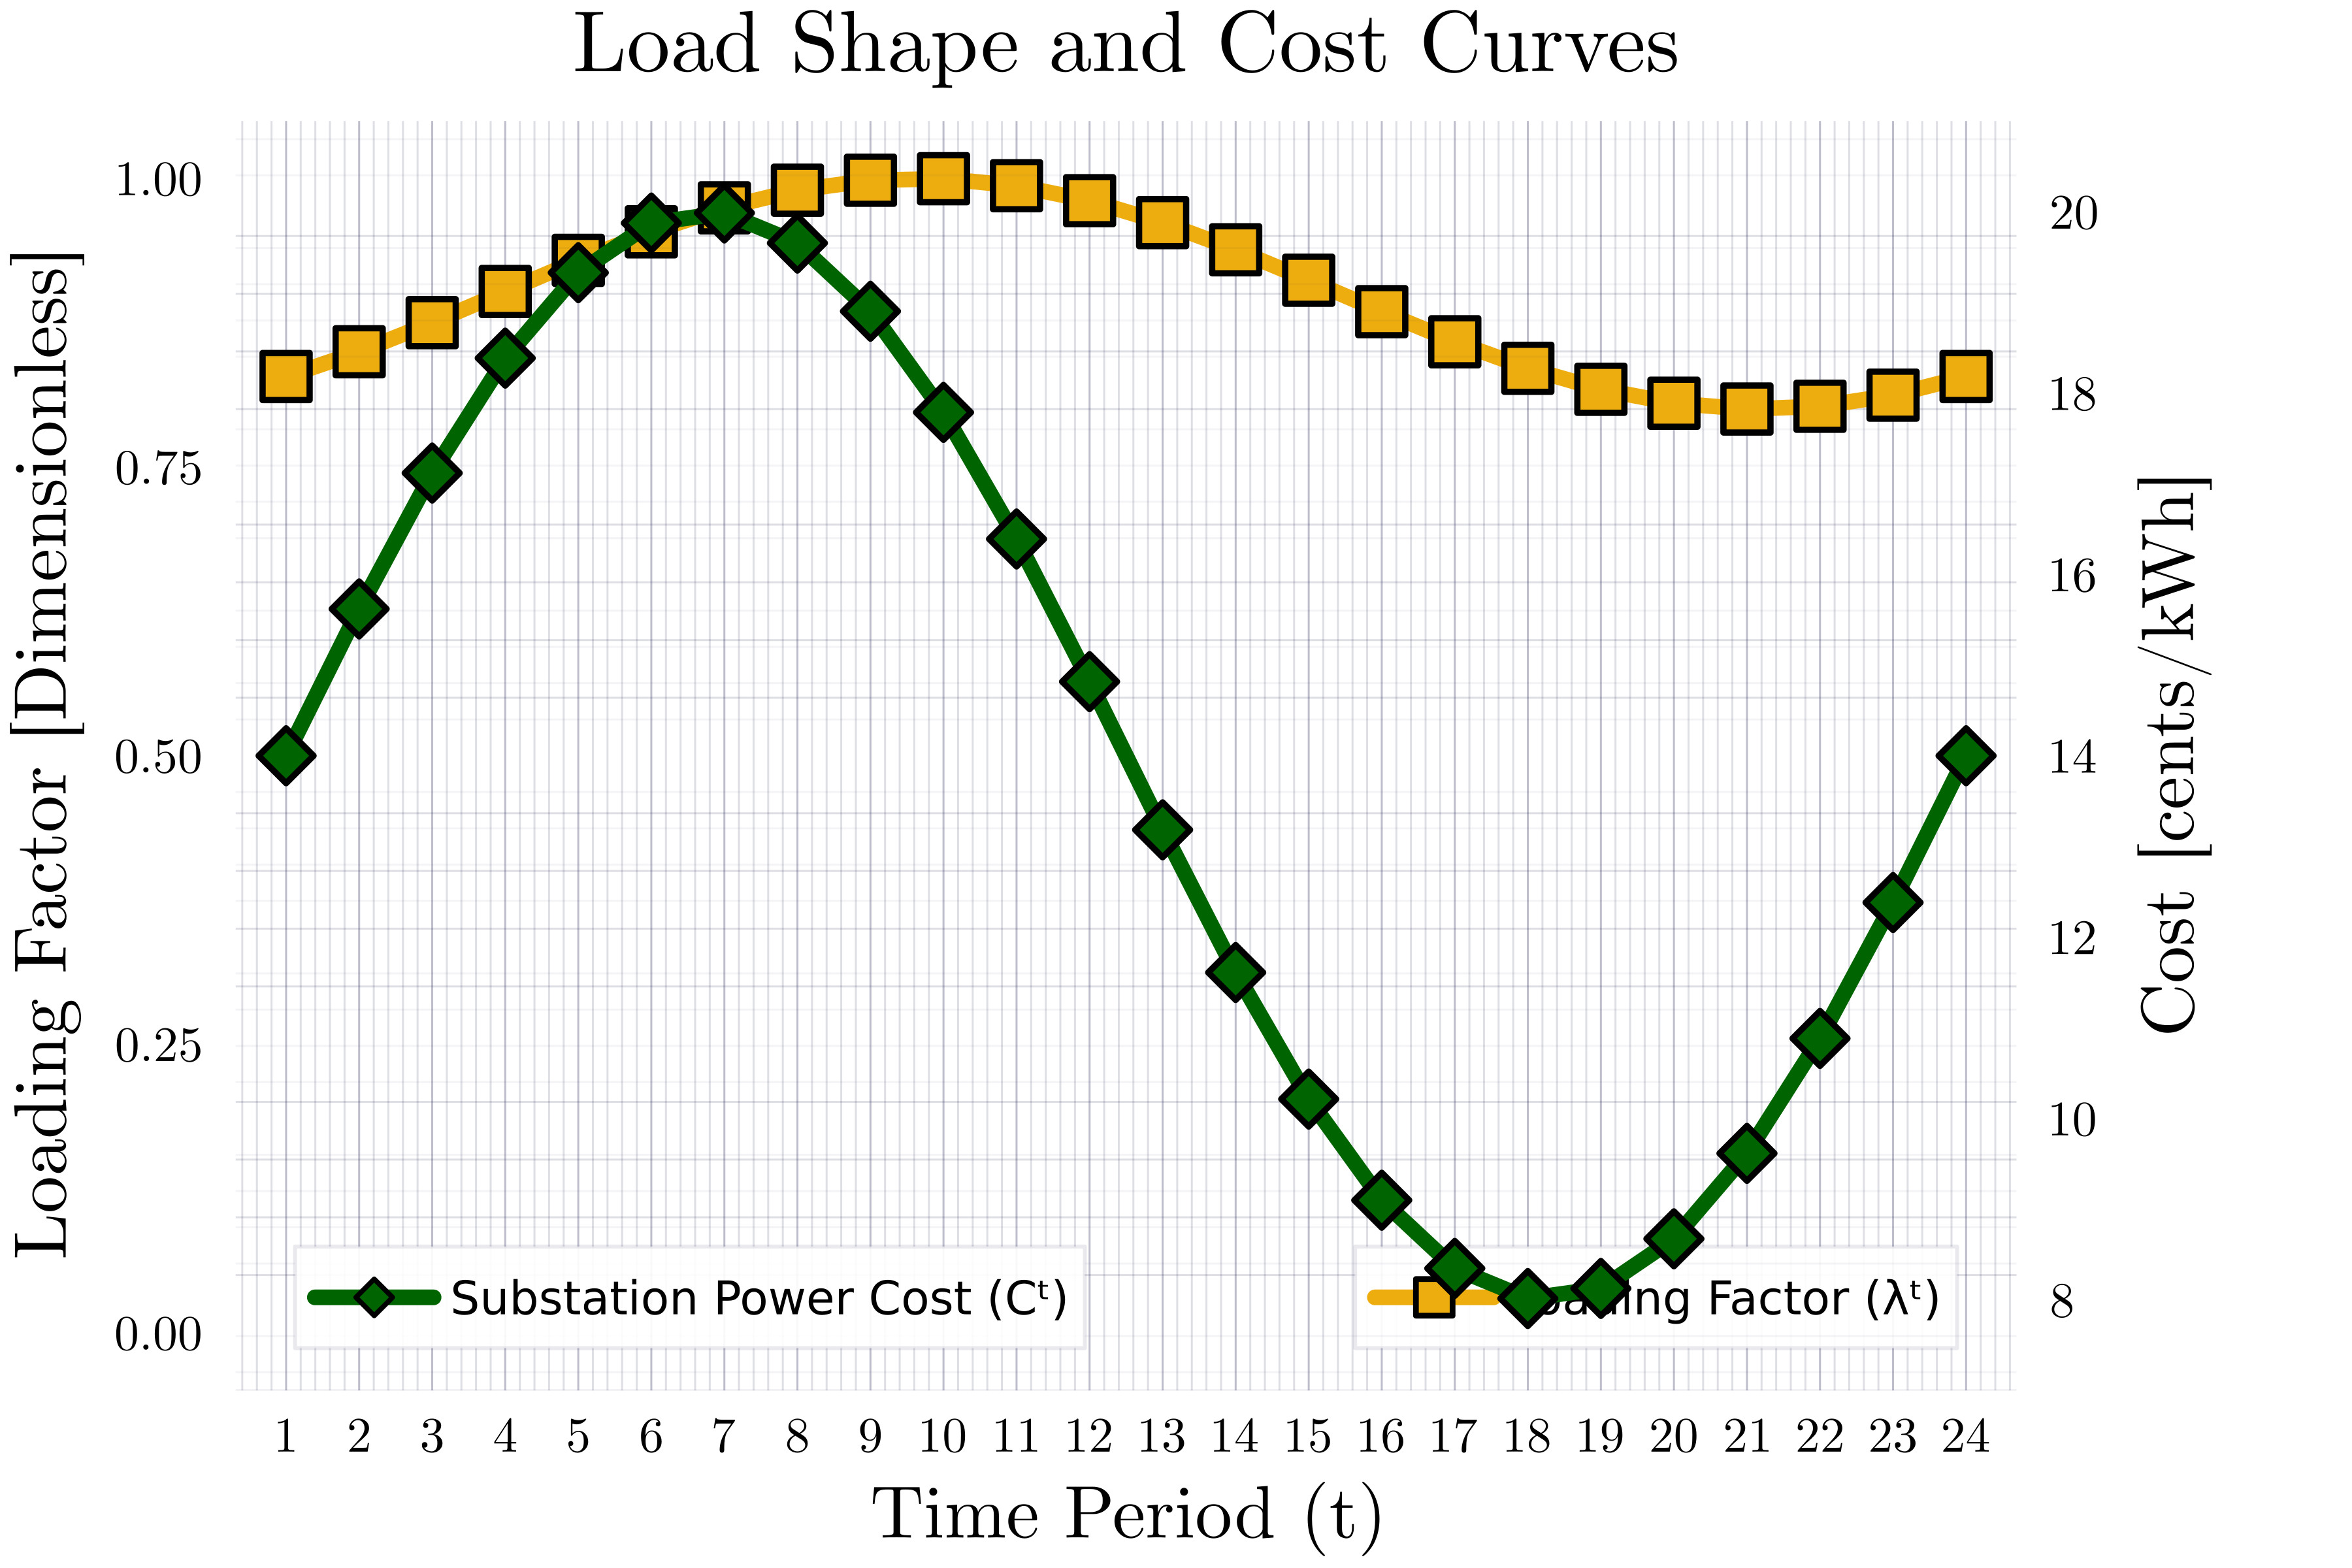
\includegraphics[width=0.7\textwidth]{figures/input-curves-cost-and-load-only-T24.png}
    \caption{Input curves showing electricity cost and load demand over a 24-hour period.}
    \label{fig:input_curves}
\end{figure}

\subsubsection{Variable Color Coding}
\begin{itemize}
    \item $B^{t_0}$: Local SOC variables for subproblem $t_0$
    \item $\hat{B}$: Global consensus SOC trajectory
    \item $u^{t_0}$: Local scaled dual variables for subproblem $t_0$
\end{itemize}

\subsubsection{tADMM Algorithm Structure}

The algorithm alternates between three update steps:

\paragraph{Step 1: Primal Update - tADMM Optimization Model}
For each subproblem $t_0 \in \{1, 2, \ldots, T\}$:

\begin{align}
\min_{P_{\text{subs}}^{t_0}, P_{B}^{t_0}, B^{t_0}} \quad & C^{t_0} \cdot P_{\text{subs}}^{t_0} + C_B \cdot \left(P_{B}^{t_0}\right)^2 + \frac{\rho}{2} \left\| B^{t_0} - \hat{B} + u^{t_0} \right\|_2^2
\end{align}

\textbf{Subject to SOC Dynamics for Entire Trajectory:}
\begin{align}
B^{t_0}[1] &= B_0 - P_{B}^{t_0} \cdot \Delta t \\
B^{t_0}[t] &= B^{t_0}[t-1] - P_{B}^{t_0} \cdot \Delta t, \quad \forall t \in \{2, \ldots, T\} \\
P_{\text{subs}}^{t_0} + P_{B}^{t_0} &= P_L[t_0] \\
-P_{B,R} \leq P_{B}^{t_0} &\leq P_{B,R} \\
\underline{B} \leq B^{t_0}[t] &\leq \overline{B}, \quad \forall t \in \{1, \ldots, T\}
\end{align}

\textbf{Key Formulation Notes:}
\begin{itemize}
    \item Each subproblem $t_0$ optimizes the battery power $P_{B}^{t_0}$ for \textit{only} time step $t_0$
    \item However, the SOC trajectory $B^{t_0}[t]$ is computed for \textit{all} time steps $t \in \{1, \ldots, T\}$
    \item This ensures that the ADMM penalty term can compare the full trajectory $B^{t_0}$ with the consensus $\hat{B}$
    \item The power balance constraint is enforced only for the specific time $t_0$
\end{itemize}

\paragraph{Step 2: Consensus Update}
\begin{align}
\hat{B}[t] &= \text{clamp}\left( \frac{1}{T} \sum_{t_0=1}^{T} \left( B^{t_0}[t] + u^{t_0}[t] \right), \underline{B}, \overline{B} \right) \\
&\quad \forall t \in \{1, 2, \ldots, T-1\} \\
\hat{B}[T] &= B_{T,\text{target}} \quad \text{(if terminal constraint exists)}
\end{align}

\paragraph{Step 3: Dual Update}
\begin{align}
u^{t_0}[t] &:= u^{t_0}[t] + \left( B^{t_0}[t] - \hat{B}[t] \right) \\
&\quad \forall t_0 \in \{1, \ldots, T\}, \, \forall t \in \{1, \ldots, T\}
\end{align}

\subsection{Numerical Results}

\subsubsection{Battery Actions and Convergence Analysis}

Fig.~\ref{fig:battery_actions_copper_plate} shows the optimal battery charging and discharging actions obtained from the copper plate tADMM formulation. The battery strategically charges during low-cost periods and discharges during high-cost periods to minimize the overall energy cost over the 24-hour horizon.

\begin{figure}[h]
    \centering
    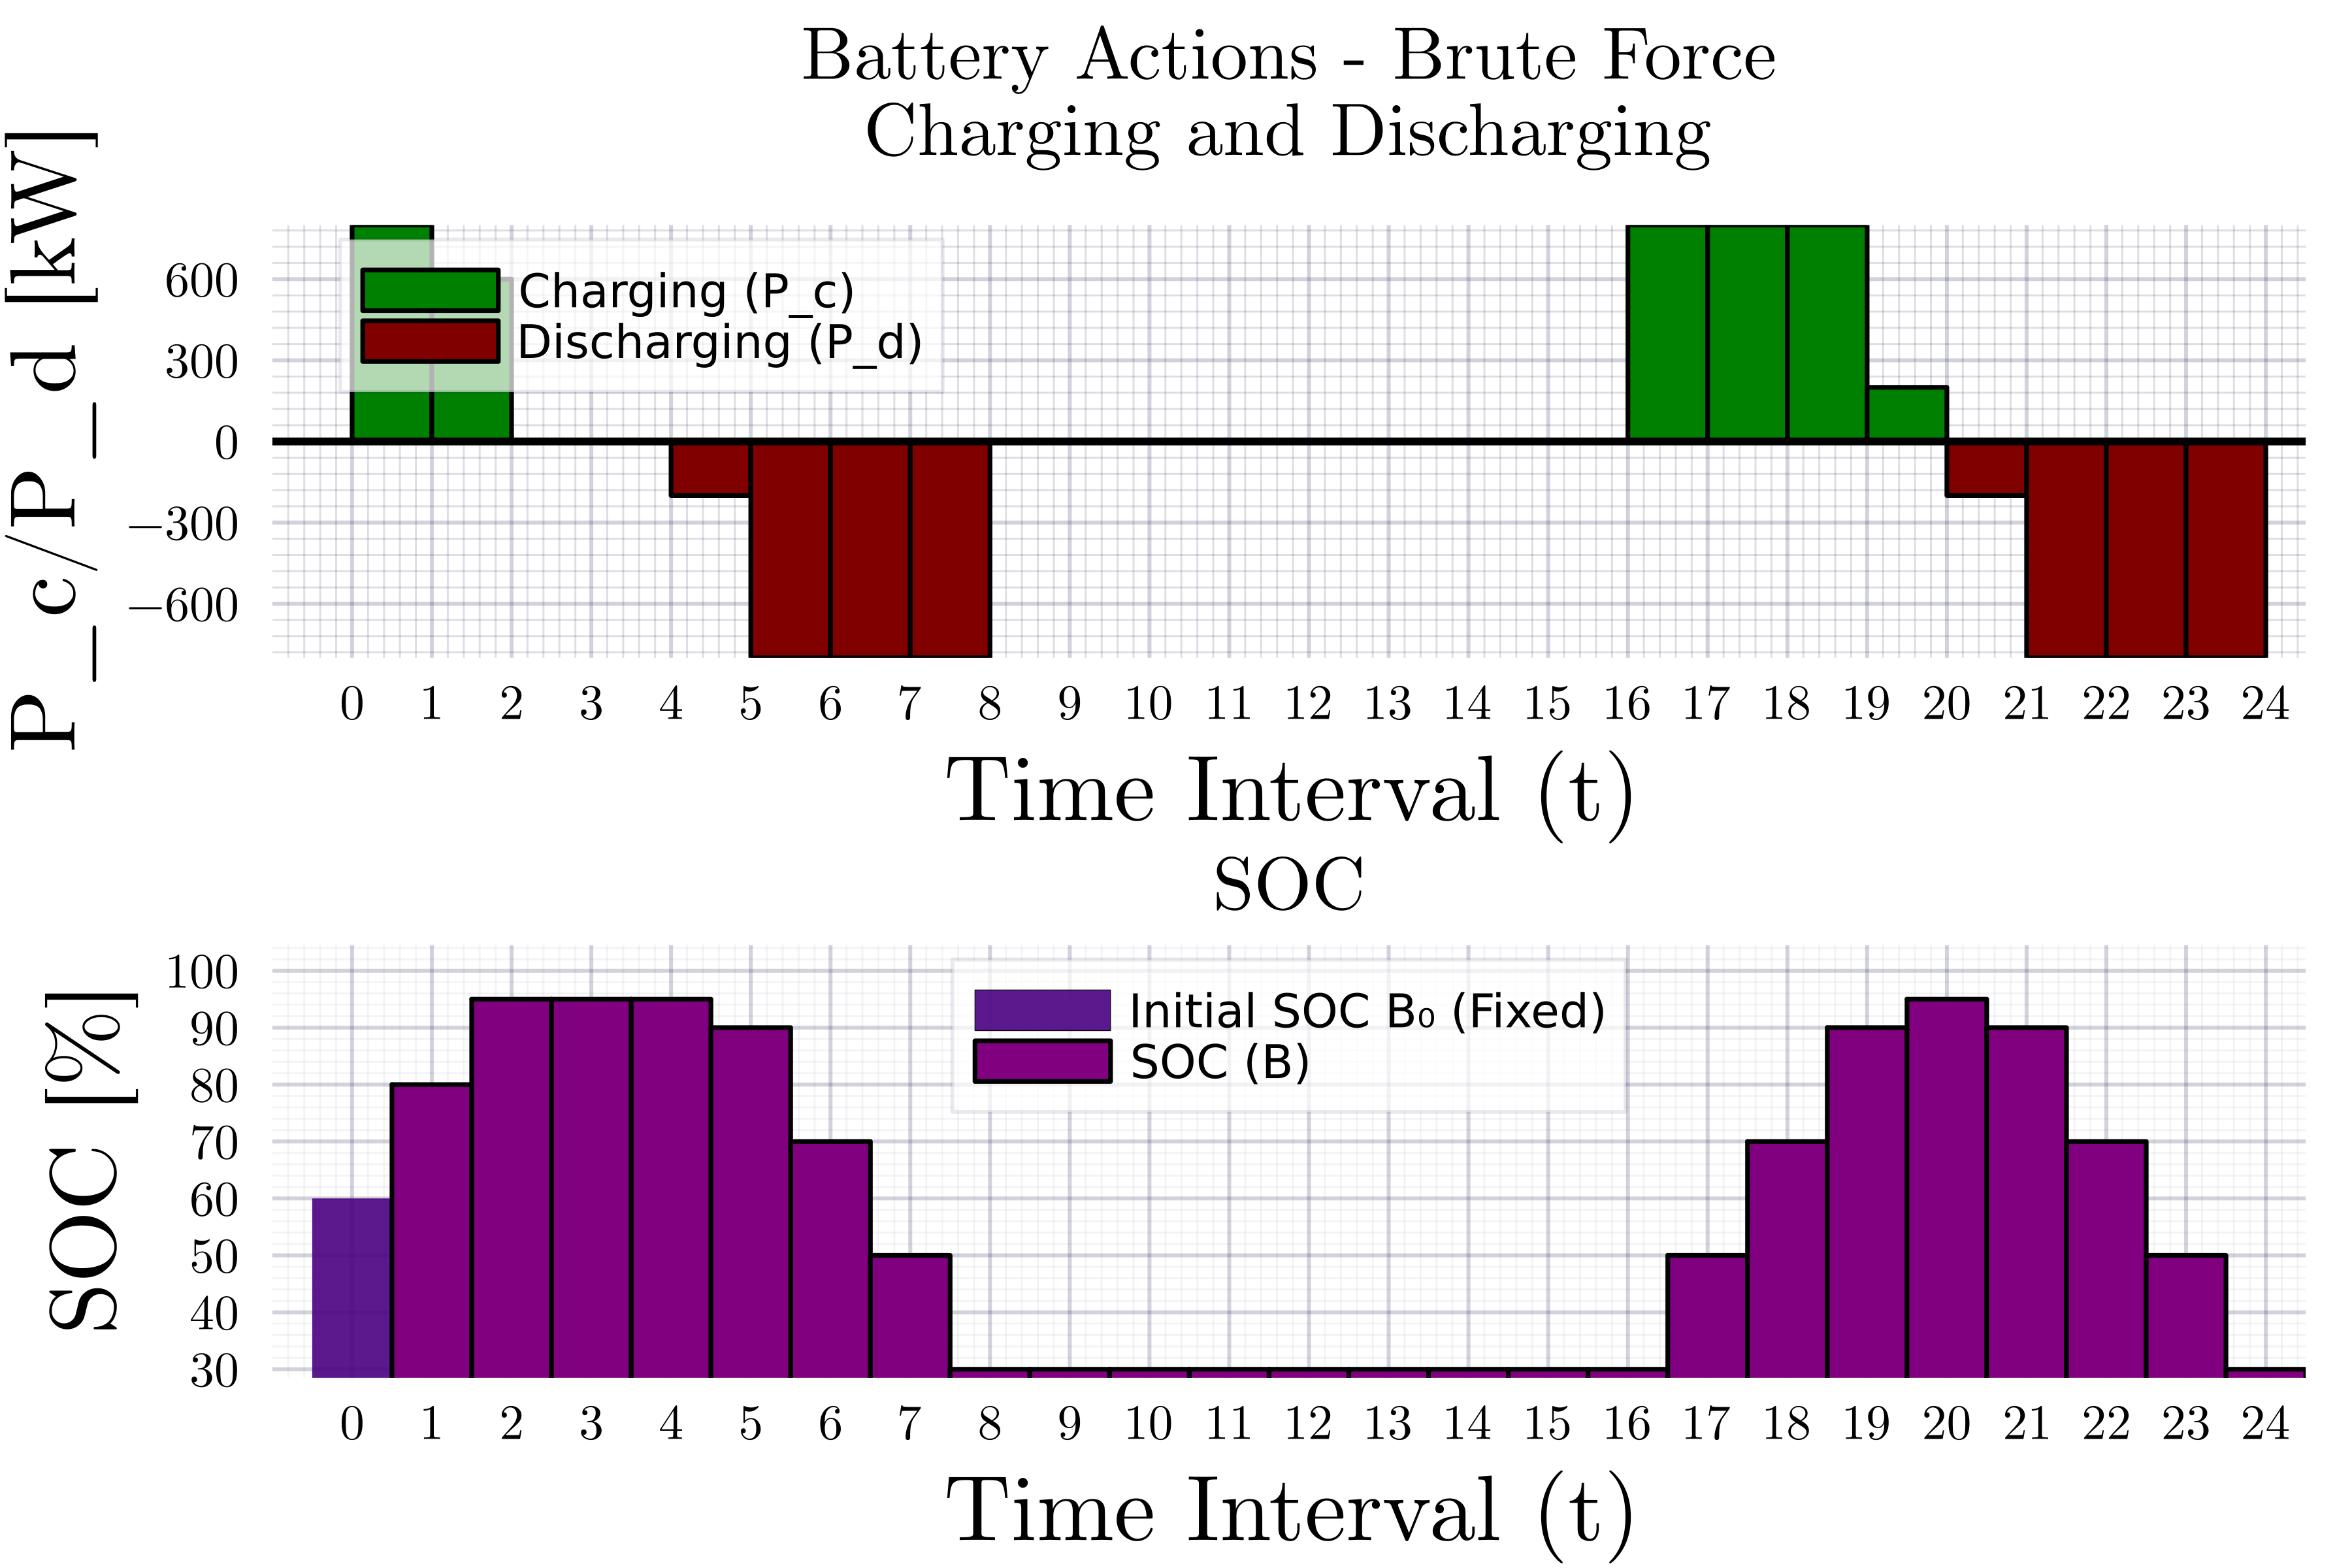
\includegraphics[width=0.7\textwidth]{figures/battery-actions-copper-plate-T24-bf.png}
    \caption{Optimal battery power actions (brute force solution) for copper plate MPOPF over 24-hour horizon.}
    \label{fig:battery_actions_copper_plate}
\end{figure}

Fig.~\ref{fig:battery_actions_tadmm} presents the battery actions obtained using the tADMM algorithm, demonstrating that the decomposition approach converges to a solution that closely matches the centralized optimal solution.

\begin{figure}[h]
    \centering
    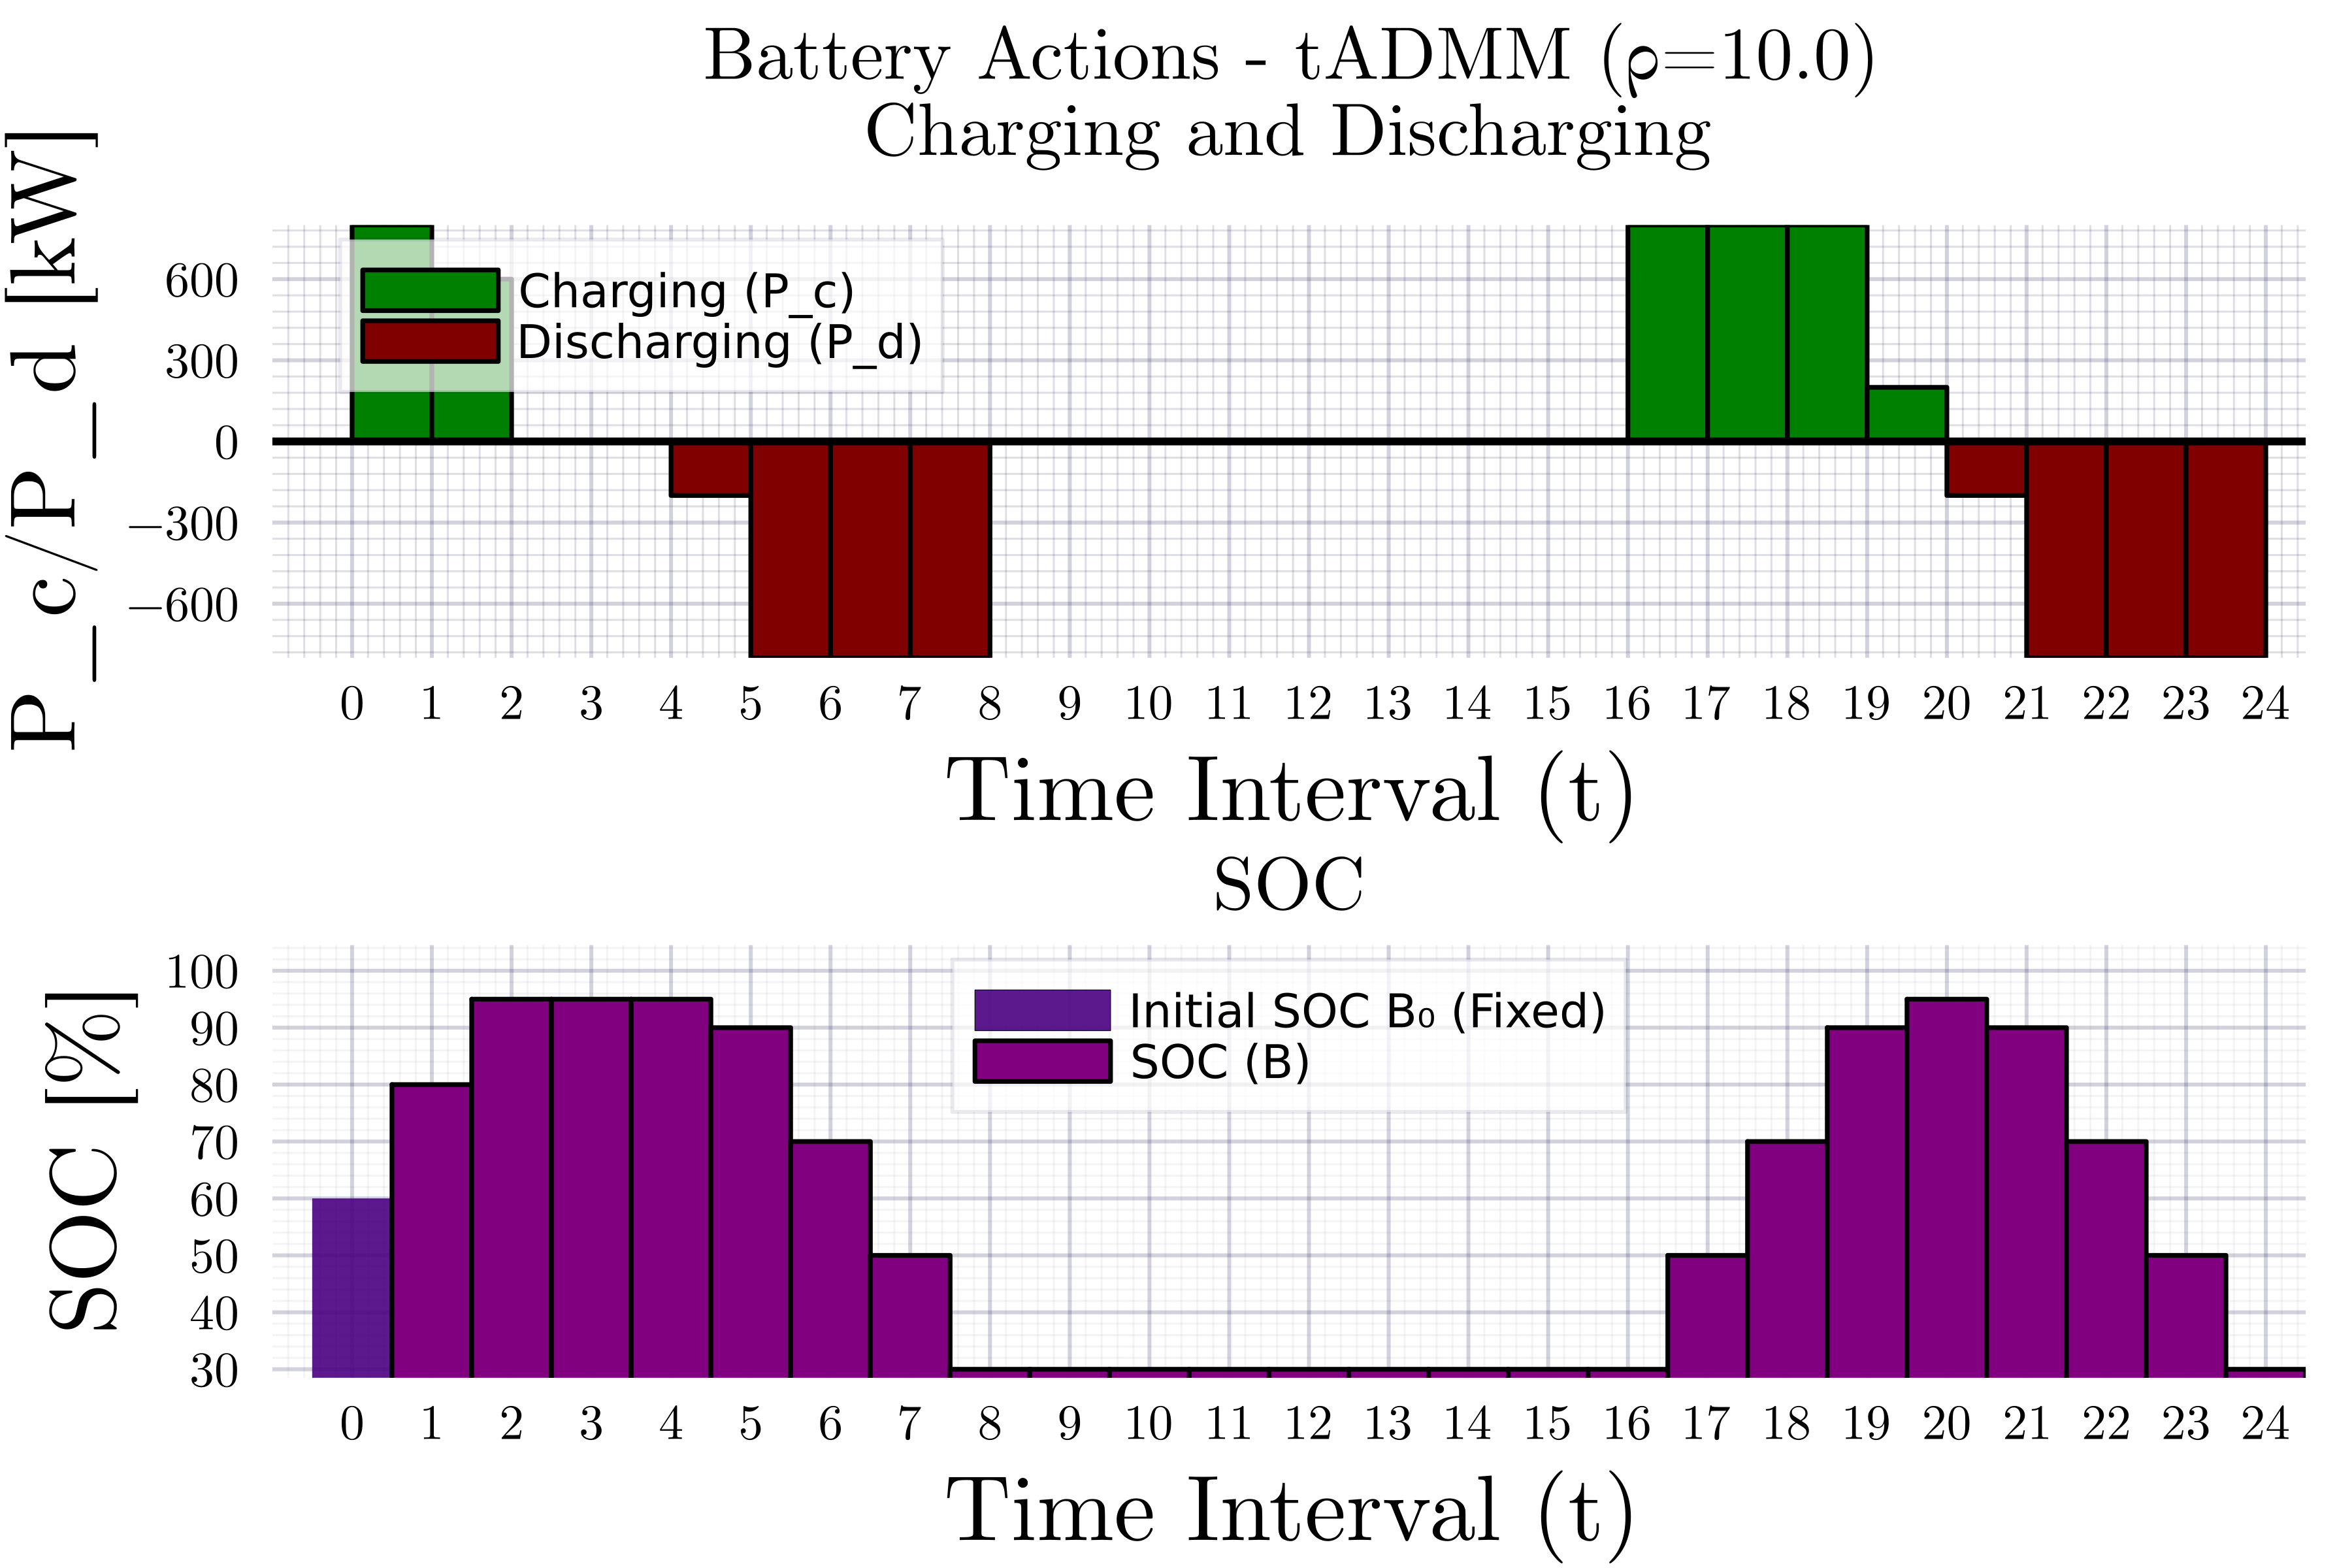
\includegraphics[width=0.7\textwidth]{figures/battery-actions-copper-plate-T24-tadmm.png}
    \caption{Battery power actions obtained using tADMM for copper plate MPOPF over 24-hour horizon.}
    \label{fig:battery_actions_tadmm}
\end{figure}

Fig.~\ref{fig:convergence_curves} illustrates the convergence behavior of the tADMM algorithm, showing how the primal and dual residuals decrease over iterations until they satisfy the specified convergence tolerances.

\begin{figure}[h]
    \centering
    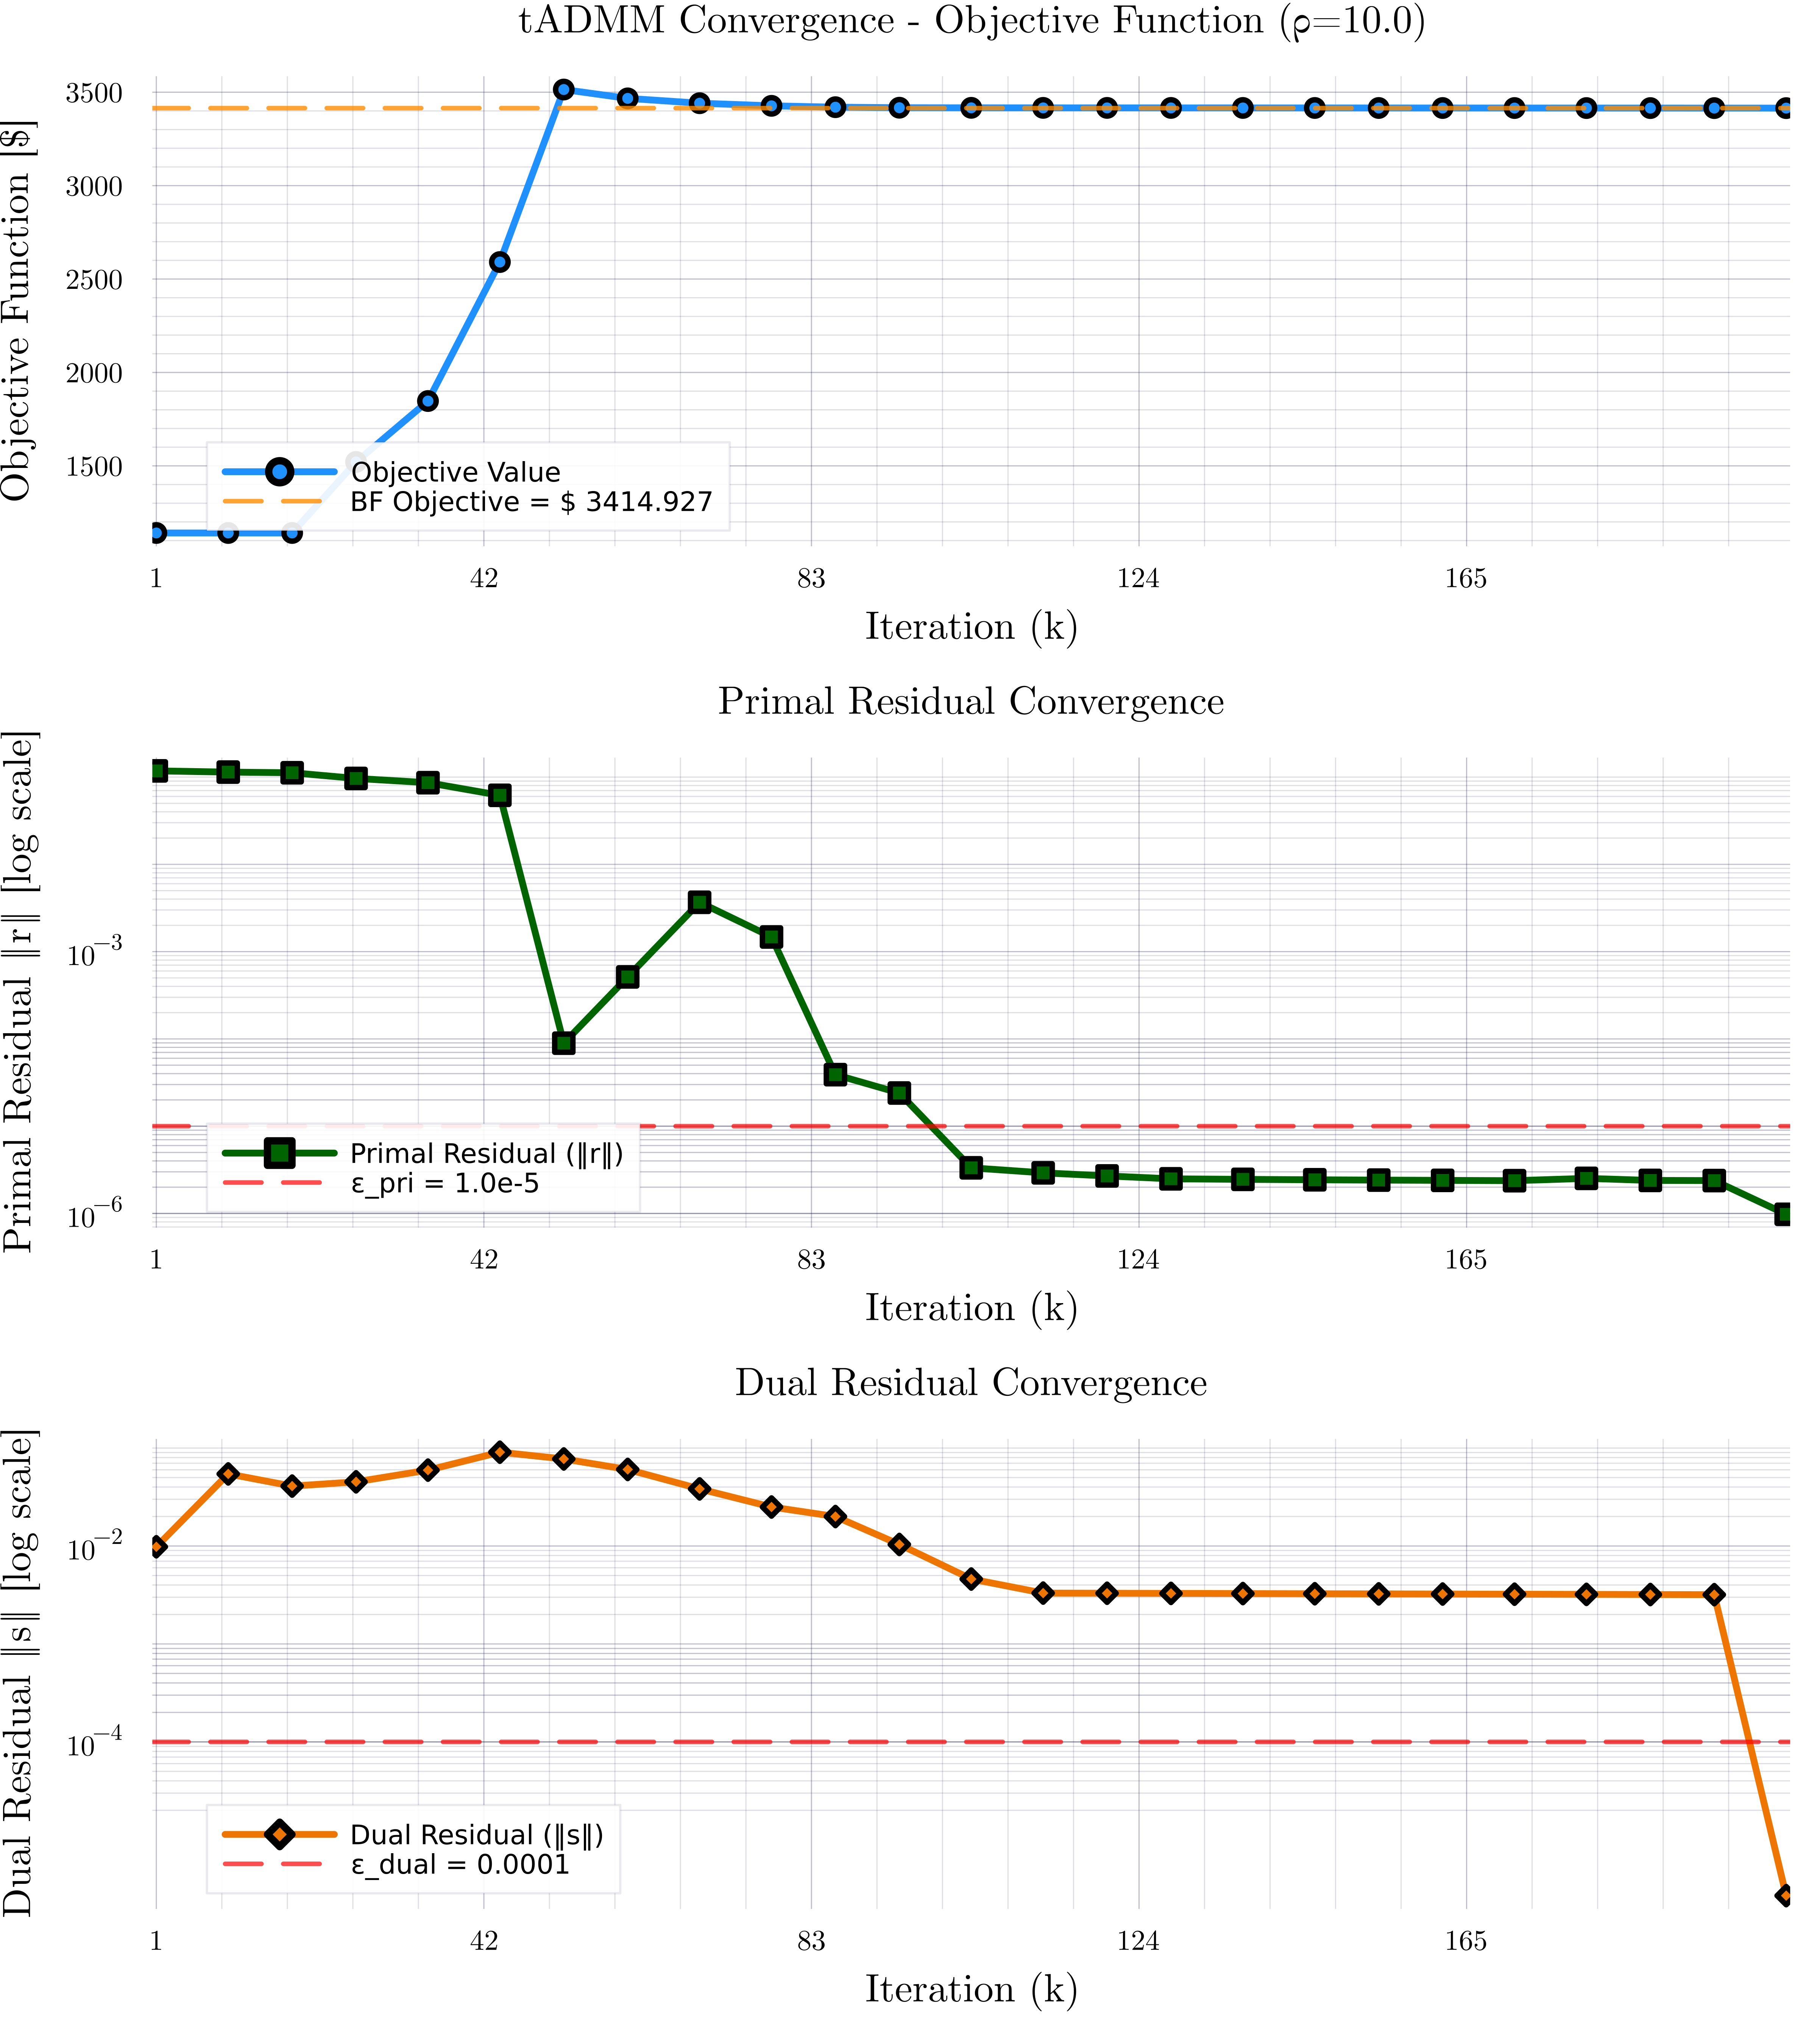
\includegraphics[width=0.7\textwidth]{figures/convergence-curves-copper-plate-T24-tadmm.png}
    \caption{Convergence curves showing primal and dual residuals for tADMM algorithm.}
    \label{fig:convergence_curves}
\end{figure}

\subsection{Convergence Criteria}

The algorithm terminates when both residuals fall below specified thresholds:

\subsubsection{Primal Residual (Consensus Violation)}
\begin{align}
\|r^k\|_2 &= \left\| \text{vec}\left( \left\{ B^{t_0} - \hat{B} \right\}_{t_0=1}^T \right) \right\|_2 \leq \epsilon_{\text{pri}}
\end{align}

\subsubsection{Dual Residual (Consensus Change)}
\begin{align}
\|s^k\|_2 &= \rho \left\| \hat{B}^k - \hat{B}^{k-1} \right\|_2 \leq \epsilon_{\text{dual}}
\end{align}

\subsection{Algorithm Parameters}

\subsubsection{Objective Function Components}

The tADMM objective function for each subproblem $t_0$ consists of three terms:

\begin{align}
\text{Energy Cost:} \quad & C^{t_0} \cdot P_{\text{subs}}^{t_0} \cdot \Delta t \\
\text{Battery Quadratic Cost:} \quad & C_B \cdot \left(P_{B}^{t_0}\right)^2 \cdot \Delta t \\
\text{ADMM Penalty:} \quad & \frac{\rho}{2} \left\| B^{t_0} - \hat{B} + u^{t_0} \right\|_2^2
\end{align}

Where:
\begin{itemize}
    \item $C^{t_0}$: Energy price at time $t_0$ [\$/kWh]
    \item $C_B$: Battery quadratic cost coefficient [\$/kW$^2$/h] (typically $10^{-6} \times \min(C^t)$)
    \item $\rho$: ADMM penalty parameter
\end{itemize}

The battery quadratic cost term $C_B \cdot \left(P_{B}^{t_0}\right)^2$ serves as a regularization to:
\begin{enumerate}
    \item Prevent excessive battery cycling
    \item Encourage smoother power trajectories
    \item Improve numerical conditioning of the optimization problem
\end{enumerate}

\subsubsection{Algorithmic Parameters}

\begin{itemize}
    \item \textbf{Penalty Parameter}: $\rho$ (typically 0.1 to 10.0)
    \item \textbf{Primal Tolerance}: $\epsilon_{\text{pri}} = 10^{-3}$
    \item \textbf{Dual Tolerance}: $\epsilon_{\text{dual}} = 10^{-3}$
    \item \textbf{Maximum Iterations}: 1000
\end{itemize}

\subsection{Appendix: Full Variable and Parameter Definitions}

\subsubsection{System Bases}
\begin{align}
\text{kV}_B &= \frac{4.16}{\sqrt{3}} \text{ kV (phase-to-neutral)} \\
\text{kVA}_B &= 1000 \text{ kVA} \\
P_{\text{BASE}} &= 1000 \text{ kW} \\
E_{\text{BASE}} &= 1000 \text{ kWh per hour}
\end{align}

\subsubsection{SOC Bound Definitions}
\begin{align}
\underline{B} &= \text{SOC}_{\min} \cdot E_{\text{Rated}} \\
\overline{B} &= \text{SOC}_{\max} \cdot E_{\text{Rated}}
\end{align}

\subsubsection{Physical Interpretation}
\begin{itemize}
    \item $P_B[t] > 0$: Battery discharging (providing power to the system)
    \item $P_B[t] < 0$: Battery charging (consuming power from the system)
    \item $B[t]$: Battery state of charge at the end of period $t$
    \item $\underline{B} = \text{SOC}_{\min} \cdot E_{\text{Rated}}$: Lower SOC bound
    \item $\overline{B} = \text{SOC}_{\max} \cdot E_{\text{Rated}}$: Upper SOC bound
\end{itemize}
